% Options for packages loaded elsewhere
\PassOptionsToPackage{unicode}{hyperref}
\PassOptionsToPackage{hyphens}{url}
%
\documentclass[
]{article}
\usepackage{amsmath,amssymb}
\usepackage{iftex}
\ifPDFTeX
  \usepackage[T1]{fontenc}
  \usepackage[utf8]{inputenc}
  \usepackage{textcomp} % provide euro and other symbols
\else % if luatex or xetex
  \usepackage{unicode-math} % this also loads fontspec
  \defaultfontfeatures{Scale=MatchLowercase}
  \defaultfontfeatures[\rmfamily]{Ligatures=TeX,Scale=1}
\fi
\usepackage{lmodern}
\ifPDFTeX\else
  % xetex/luatex font selection
\fi
% Use upquote if available, for straight quotes in verbatim environments
\IfFileExists{upquote.sty}{\usepackage{upquote}}{}
\IfFileExists{microtype.sty}{% use microtype if available
  \usepackage[]{microtype}
  \UseMicrotypeSet[protrusion]{basicmath} % disable protrusion for tt fonts
}{}
\makeatletter
\@ifundefined{KOMAClassName}{% if non-KOMA class
  \IfFileExists{parskip.sty}{%
    \usepackage{parskip}
  }{% else
    \setlength{\parindent}{0pt}
    \setlength{\parskip}{6pt plus 2pt minus 1pt}}
}{% if KOMA class
  \KOMAoptions{parskip=half}}
\makeatother
\usepackage{xcolor}
\usepackage[margin=1in]{geometry}
\usepackage{graphicx}
\makeatletter
\def\maxwidth{\ifdim\Gin@nat@width>\linewidth\linewidth\else\Gin@nat@width\fi}
\def\maxheight{\ifdim\Gin@nat@height>\textheight\textheight\else\Gin@nat@height\fi}
\makeatother
% Scale images if necessary, so that they will not overflow the page
% margins by default, and it is still possible to overwrite the defaults
% using explicit options in \includegraphics[width, height, ...]{}
\setkeys{Gin}{width=\maxwidth,height=\maxheight,keepaspectratio}
% Set default figure placement to htbp
\makeatletter
\def\fps@figure{htbp}
\makeatother
\setlength{\emergencystretch}{3em} % prevent overfull lines
\providecommand{\tightlist}{%
  \setlength{\itemsep}{0pt}\setlength{\parskip}{0pt}}
\setcounter{secnumdepth}{-\maxdimen} % remove section numbering
\ifLuaTeX
  \usepackage{selnolig}  % disable illegal ligatures
\fi
\IfFileExists{bookmark.sty}{\usepackage{bookmark}}{\usepackage{hyperref}}
\IfFileExists{xurl.sty}{\usepackage{xurl}}{} % add URL line breaks if available
\urlstyle{same}
\hypersetup{
  hidelinks,
  pdfcreator={LaTeX via pandoc}}

\author{}
\date{\vspace{-2.5em}}

\begin{document}

\hypertarget{results}{%
\section{Results}\label{results}}

\hypertarget{statistical-analysis}{%
\subsection{Statistical Analysis}\label{statistical-analysis}}

\subsection*{Calculation of Ash-Free Dry Weight (AFDW):}

The AFDW was determined using the following equation:

\[
AFDW = DW \times \left(1 - \frac{{\text{Ash Content}}}{{100}}\right)
\]

\begin{itemize}
    \item \( AFDW \): Ash-free dry weight.
    \item \( DW \): Dry weight of the sample.
    \item \text{Ash Content}: Percentage of ash content in the sample.
\end{itemize}

\subsection*{Conversion of Oxygen Consumption to Energy Expenditure:}

~~~~~ Cellular respiration involves the consumption of oxygen (O2)
through a process of organismal respiration to produce energy in the
form of adenosine triphosphate (ATP) \cite{babcock1992oxygen} according
to the equation:

\[
C_6H_{12}O_6 + 6O_2 \rightarrow 6CO_2 + 6H_2O + \text{energy (as ATP)}
\]

~~~~~ To calculate respiration, we first multiplied the moles of oxygen
consumed per hour by the molar mass of oxygen, which is approximately
\(32 \, \text{g/mol}\) \citep{hochachka1983protons}, to convert from
moles of oxygen to grams of oxygen. Then we used an oxy-joulometric
conversion factor derived from \cite{elliott1975energy}, which is
\(14.14 \, \text{J/mg O}_2\), to convert from grams of oxygen consumed
per hour to joules of energy expended during cellular respiration.

The calculation can be expressed as follows:

\[
\text{Energy expenditure (J)} = \text{grams of O}_2 \times \text{conversion factor}
\]

To convert moles of oxygen to grams, we used the molar mass of oxygen:

\[
\text{grams of O}_2 = \text{moles of O}_2 \times 32 \, \text{g/mol}
\]

Substituting the values, we get:

\[
\text{Energy expenditure (J)} = \text{grams of O}_2 \times 14140 \, \text{J/g O}_2
\]

where \(32 \, \text{g/mol}\) is the molar mass of oxygen and
\(14140 \, \text{J/g O}_2\) is the conversion factor derived from
\cite{elliott1975energy} and expressed as \(14.140 \, \text{J/mg O}_2\)
before conversion.

~~~~~ After converting the oxygen consumption rates to energy
expenditure in joules per hour per snail and performing statistical
analysis, we conducted a two-way ANOVA to investigate the effects of
temperature treatment and pH treatment on energy expenditure. The ANOVA
revealed a significant effect of temperature treatment (\(p < 0.001\)),
indicating that different temperature treatments had a significant
impact on energy expenditure. Although the pH treatment showed some
effect on energy expenditure, it was marginally significant (F(1, 44) =
3.9760, p = 0.05237), suggesting a potential influence of pH on energy
expenditure. The interaction between temperature and pH treatment was
not significant (F(7, 44) = 1.5286, p = 0.18280), indicating that the
combined effect of temperature and pH treatment did not significantly
impact energy expenditure beyond the individual effects of each factor.
Subsequent Tukey multiple comparisons showed significant differences
between most temperature treatment pairs. For example, the energy
expenditure at 14°C was significantly higher than at 12°C (mean
difference = 13.31 J/h, p \textless{} 0.001), and the energy expenditure
at 22°C was significantly higher than at 20°C (mean difference = 60.21
J/h, p \textless{} 0.001). Tukey multiple comparison indicated a
significant difference between low and ambient pH conditions, with a
higher energy expenditure observed under low pH (mean difference = 5.95
J/h, p \textless{} 0.001).

\begin{table}[htbp]
    \centering
    \caption{Energy Expenditure at Different Temperatures for Ambient and Low pH Treatments}
    \label{table3}
    \begin{tabular}{cccc}
    \toprule
    Temperature & Treatment & Energy Expenditure (J/h) & Percent Difference \\
    \midrule
    12 & Ambient & 20.68363 & -10.28\% \\
    & Low & 23.05466 & \\
    14 & Ambient & 33.82566 & -8.28\% \\
    & Low & 36.88008 & \\
    16 & Ambient & 33.41744 & -19.53\% \\
    & Low & 41.52857 & \\
    18 & Ambient & 68.02335 & 19.56\% \\
    & Low & 56.89424 & \\
    20 & Ambient & 69.03278 & -4.30\% \\
    & Low & 72.13377 & \\
    22 & Ambient & 58.85060 & -37.60\% \\
    & Low & 94.31767 & \\
    24 & Ambient & 85.51626 & -20.26\% \\
    & Low & 107.24288 & \\
    26 & Ambient & 53.82479 & -5.62\% \\
    & Low & 57.03218 & \\
    \bottomrule
    \end{tabular}
\end{table}

\newpage

\subsection*{Thermal Performance Curve Analysis:}

~~~~~ All statistical analyses were run in the R environment
\citep{R_core_team_2021}. The \textit{rTPC} \citep{padfield2021rtpc} and
\textit{nls.multstart} packages were used to fit a series of models to
the respiration rate data and build thermal performance curves. The
analysis utilized the \textit{rtpc} package in R, which enables a
pipeline to fit data to multiple models simultaneously. Thermal
performance curves (TPC) were analyzed to investigate the relationship
between temperature and performance measure (e.g., metabolic rate) of
\textit{T. funebralis}. The statistical processing of the thermal
performance curves involved analyzing the data collected from the
respiration chambers and examining statistical graphs of oxygen
evolution over time. Regression analysis was employed to explore the
relationship between temperature and oxygen evolution and to estimate
the parameters of the thermal performance curve (e.g., slope).
Specifically, we have utilized techniques such as nonlinear regression
to fit thermal performance models to the data and assess the goodness of
fit.

~~~~~ During the regression analysis, it was crucial to examine the
distribution of model parameters this involved assessing the normality
of the distribution of \(\beta\) values and investigating potential
outliers or unusual patterns.Additionally, we inspected the distribution
of residuals, which are the differences between observed and predicted
values, to ensure they were normally distributed and exhibited
homoscedasticity. Additionally, diagnostic plots, specifically
quantile-quantile (Q-Q) plots, were employed to assess the normality of
residuals and identify any potential outliers or systematic patterns
embedded within the data. We examined the relationship between predictor
variables (e.g., temperature) and fitted values to ensure the model
adequately captured the underlying trends in the data. Moreover, we
inspected the standard residuals, to identify observations with
unusually large or small residuals. Any outlying observations that
indicated data errors, measurement inaccuracies, or other anomalies that
necessitated further investigation were subsequently excluded from the
analysis.

\newpage

\subsection*{Model Fit and Selection:}

~~~~~ The thermal performance curve (TPC) model was fitted to the data
using nonlinear regression techniques in R, specifically the
\texttt{nls\_multistart()} function. Model fit was assessed with the
coefficient of determination (\(R^2\)), indicating a strong fit to the
observed data. The model selection process involved fitting several
models for ectotherm physiology (e.g., Gaussian, Sharpe-Schoolfield)
using Akaike Information Criterion corrected for small sample sizes
(AICc). The Sharpe-Schoolfield model was chosen as the preferred model
for this study due to its goodness of fit, and its physiological
relevance to ectotherms based on enzyme kinetics. This model is widely
used in ecological and physiological studies to understand how organisms
respond to changing environmental temperatures, particularly in the
context of climate change and thermal stress.Additionally, bootstrap
resampling methods were employed to assess parameter uncertainty and
validate the uncertainty of the data following
\cite{Olito2017estimating}.

\textbf{Sharpe-Schoolfield High Model Equation:} \begin{equation}
R(T) = \frac{R_{\text{ref}}}{1 + e^{\left(\frac{E}{k}\left(\frac{1}{T} - \frac{1}{T_{\text{ref}}}\right)\right) + e_h\left(\frac{1}{T} - \frac{1}{T_{\text{opt}}}\right)}}
\end{equation}

\textbf{Description of Variables:}

\begin{itemize}
    \item \( R(T) \): Rate of the biological process at temperature \( T \).
    \item \( R_{\text{ref}} \): Rate at the standardised temperature, \( T_{\text{ref}} \).
    \item \( E \): Activation energy (eV).
    \item \( k \): Boltzmann's constant (\( 8.617333262145 \times 10^{-5} \) eV/K).
    \item \( T \): Temperature (°C).
    \item \( T_{\text{ref}} \): Standardisation temperature (°C). Temperature at which rates are not inactivated by either high or low temperatures.
    \item \( e_h \): High temperature deactivation energy (eV).
    \item \( T_{\text{opt}} \): Temperature (°C) at which enzyme is 1/2 active and 1/2 suppressed due to high temperatures.
\end{itemize}

\textbf{Additional Information:} The Sharpe-Schoolfield high model
describes the temperature dependence of biological rates, such as
metabolic rates, enzyme activities, or reaction rates, in response to
high temperatures. It incorporates parameters such as activation energy,
high temperature deactivation energy, and optimum temperature to
characterize the thermal performance curve \cite{sharpe1981non}. The
results of the thermal performance curve analysis provide insights into
the organism's temperature-dependent performance and its thermal
ecology. The optimum temperature (Topt) indicates the temperature range
in which the organism performs optimally, while the thermal limits
(CTmin and CTmax) define the species' thermal tolerance. The thermal
sensitivity or breadth parameter (b) reflects the organism's ability to
acclimate or adapt to temperature changes and its vulnerability to
thermal stress.

\begin{figure}[htbp]
  \centering
  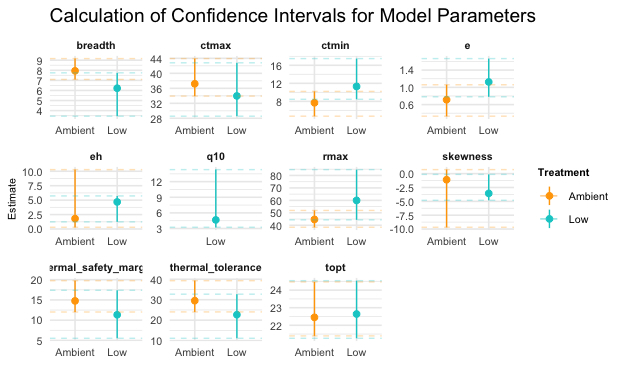
\includegraphics[width=0.8\textwidth]{Images/params.jpg}
  \caption{Extracted thermal performance parameters and metrics for \textit{Tegula funebralis}, indicating no statistical difference between the thermal performance curves (TPCs) under ocean acidification (OA) treatment overall for all TPC parameters.}
  \label{fig:tpc-params}
\end{figure}

\begin{figure}[htbp]
  \centering
  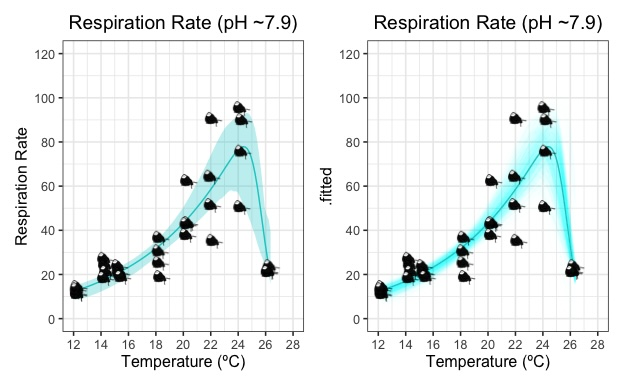
\includegraphics[width=0.8\textwidth]{Images/schoolfield-high.jpg}
  \caption{Thermal performance curve of \textit{Tegula funebralis}, depicting individuals' respiration rates (in $\mu mol$ O$_2$ per gram of ash-free dry weight) across temperatures ranging from 12°C to 26°C at a pH of 7.9 $\pm$ 0.1. One plot includes bootstraps while the other presents calculated confidence intervals. The plot was generated using the \texttt{rtpc} package in R \citep{padfield2021rtpc}.}
This caption provides a clear description of the figure, including the species studied, the 
  \label{fig:tpc-schoolfield-high}
\end{figure}

\begin{figure}[htbp]
  \centering
  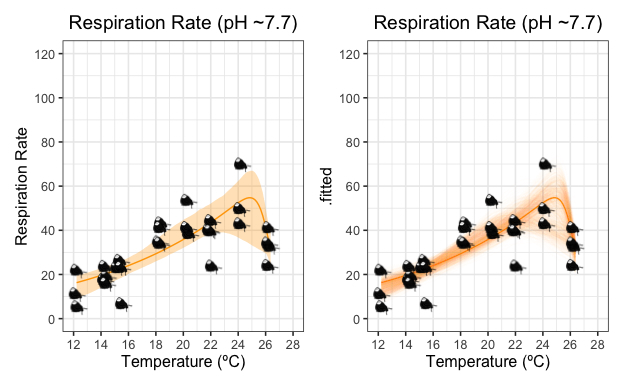
\includegraphics[width=0.8\textwidth]{Images/schoolfield-low.jpg}
  \caption{Thermal performance curve of \textit{Tegula funebralis}, depicting individuals' respiration rates (in $\mu mol$ O$_2$ per gram of ash-free dry weight) across temperatures ranging from 12°C to 26°C at a pH of 7.7 $\pm$ 0.8. One plot includes bootstraps while the other presents calculated confidence intervals. The plot was generated using the \texttt{rtpc} package in R \citep{padfield2021rtpc}.}
  \label{fig:tpc-schoolfield-low}
\end{figure}

\end{document}
